\documentclass{article}

% Language setting
% Replace `english' with e.g. `spanish' to change the document language
\usepackage[russian]{babel}
\usepackage{amsmath}

%графика
\usepackage{wrapfig}
\usepackage{graphicx}
\usepackage{pgfplots}
\usepackage{tikz}


\usepackage{tcolorbox}

% Set page size and margins
% Replace `letterpaper' with `a4paper' for UK/EU standard size
\usepackage[letterpaper,top=2cm,bottom=2cm,left=3cm,right=3cm,marginparwidth=1.75cm]{geometry}

% Useful packages
\usepackage{amsmath}
\usepackage{amssymb}
\usepackage{graphicx}
\usepackage{fixltx2e}
\usepackage[colorlinks=true, allcolors=blue]{hyperref}
\usepackage{subcaption}
\usepackage{caption}

\usepackage{hyperref}

\usepackage{makecell}
\renewcommand\theadalign{bc}
\renewcommand\theadfont{\bfseries}
\renewcommand\theadgape{\Gape[4pt]}
\renewcommand\cellgape{\Gape[4pt]}

\usepackage{geometry}
\geometry{left=25mm,right=25mm,
 top=25mm,bottom=25mm}

\newcommand{\specialcell} [2] [c] { {% 
		\def\arraystretch{2}%
		\begin{tabular} [#1] {@{}c@{}} #2 \end{tabular}}}

\title{Quantitative Analytics.\\
Lectures. Week 3. \\
Option Sensitivities Measures The Greeks. Греки или меры чувствительности опционов к изменению параметров.}
\author{Akhundzhanova Elina}

% Колонтитулы
\usepackage{fancyhdr}
\pagestyle{fancy}
\renewcommand{\headrulewidth}{0.1mm}  
\renewcommand{\footrulewidth}{0.1mm}
\lfoot{}
\rfoot{\thepage}
\cfoot{}
\rhead{CMF-2022}
\chead{}
%\renewcommand{\figurename}{Рис.}

\begin{document}
\maketitle

% Оглавление
\setcounter{tocdepth}{2} % - в оглавлении участвуют chapter, section и subsection. {1} - только chapter и section
\renewcommand\contentsname{Содержание}
\tableofcontents
\newpage

% \section{Dictionary, Definitions, Abbreviations}

% \subsection{Dictionary}
% \begin{itemize}
%     \item IR - Interest rate - процентная ставка.
%     \item Compounding - платежи (idk)
% \end{itemize}

% \subsection{Definitions and Abbreviations}
% \begin{itemize}
%     \item SAR - Stated annual rate.
%     \item EAR - Effective annual rate.
%     \item FoC - Frequency of Compounding
%     \item PMT - Payment
%     \item r - Interest rate (at the moment). 
% \end{itemize}

\renewcommand{\labelitemi}{\tiny$\bullet$}
\renewcommand{\figurename}{Рис.}

 \section{Стратегии хеджирования}
 \subsection{Непокрытая, покрытая и stop-loss стратегии}
 \begin{itemize}
     \item \textbf{Непокрытая стратегия (naked position)} означает продажу Call опциона без приобретения соответствующего underlying \ (базового) актива. \\
     \underline{Какие риски возникают?} В случае, если базовый актив в дату экспирации опциона сильно вырос в цене, тогда у нас, как у стороны, продавшей опцион, возникает обязанность доставить базовый актив по цене страйк. Так как у нас нет базового актива, то необходимо купить его на рынке по сильно выросшей цене, то есть мы имеем потенциально неограниченные убытки в рамках данной стратегии. 

     \item \textbf{Покрытая стратегия (covered position)} подразумевает продажу Call опциона и одновременно покупку базового актива. \\
      \underline{Какие риски возникают?} Риски здесь реализуются, если экспирация опциона происходит в области out-of-the-money ("вне денег"\ или "без денег").  Когда базовый актив является акцией, то у нас ограниченный downside (потенциал падения), так как цена не может быть отрицательной, но при приближении цены к 0 убытки могут существенно превысить премию от продажи опциона.
    \end{itemize}

     \underline{Возможно ли совместить стратегии naked и covered в одной?} Да, рассмотрим следующую стратегию:
     	\begin{itemize}
     \item \textbf{Стратегия stop-loss} спроектирована так, чтобы ограничить убытки от коротких позиций в опционах. Стратегия заключается в том, что если цена базового актива в области in-the-money ("в деньгах") для позиции Call, то стратегия подразумевает покупку базового актива (то есть в in-the-money области это covered позиция). Если базовый актив в области out-of-the-money (то есть ниже, чем страйк), то в данном случае происходит продажа базового актива.
     
     \begin{figure}[h]
     	\centering
     	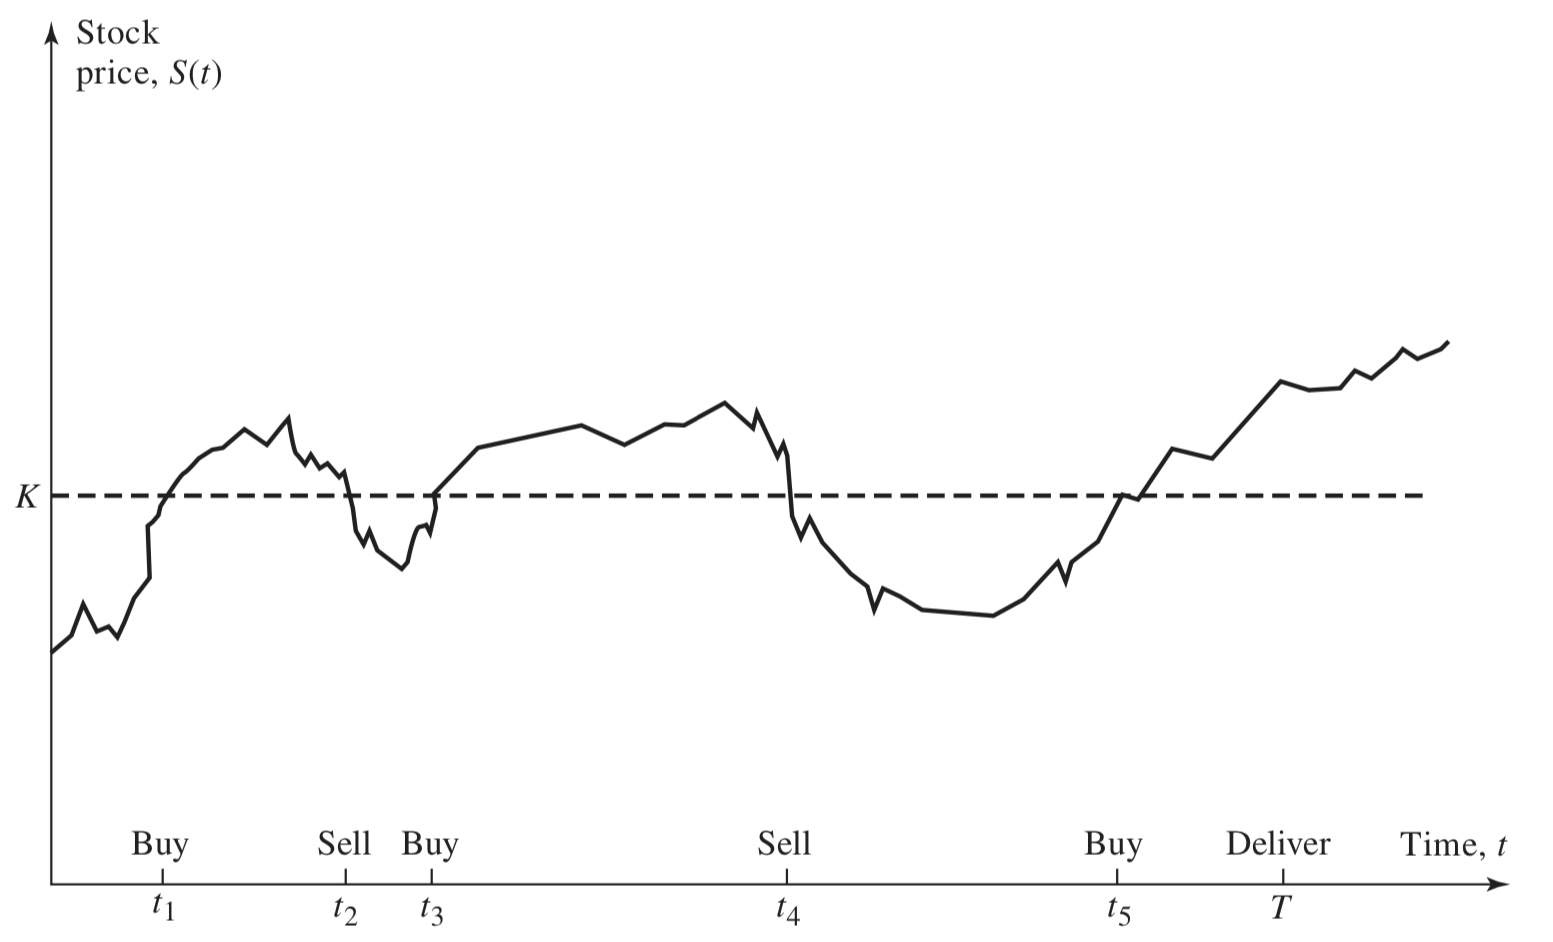
\includegraphics[width=0.7\textwidth]{Стратегия stop-loss.jpg}
     	\caption{Стратегия stop-loss}
     	\label{model}
     \end{figure}
 \end{itemize}

 Эта стратегия предполагает, что если в момент экспирации $T$ мы оказываемся в области in-the-money, то автоматически имеется базовый актив, который можно доставить. Если мы оказываемся в области out-of-the-money, то нет базового актива, который и не нужен.
 
\underline{В чем подвох данной стратегии?} Проблема в том, что при приближении к уровню страйк цены, необходимо выбрать такое $\varepsilon$, начиная с которого будет осуществляться продажа или покупка базового актива. Как только $\varepsilon \rightarrow 0$, сразу же транзакционные издержки данной стратегии увеличиваются, и нивелируются все ее преимущества.


\subsection{Дельта-нейтральная стратегия}
\begin{itemize}
	\item \textbf{Основная идея:} прибыль по опционной позиции должна компенсироваться убытком по позиции базового актива, а убыток по опционной позиции должен компенсироваться прибылью по позиции базового актива.
	
	\item \textbf{Цель:} комбинировать позицию в базовом активе с позицией в опционе на этот базовый актив так, что стоимость (value) портфеля при бесконечно малом изменении цены базового актива не меняется.
	
	\item \textbf{Важно помнить:} \hyperlink{pdf}{Дельта} (см. определение внизу страницы) опциона меняется в случае изменения цены базового актива, а также если меняется время до экспирации опциона. В таком случае необходимо периодически (чем чаще,  тем лучше в рамках стратегии) перестраивать портфель, то есть менять количество базового актива в нашем комбинированном портфеле.
	
	\item Когда выполняются предпосылки модели Блэка-Шоулза-Мёртона, то стоимость (cost) данной стратегии, дисконтированной в момент времени 0, представляет собой цену опциона по модели Блэка-Шоулза-Мёртона.
	
	\item Косты (costs) в данной стратегии практически неизбежны, так как если цена базового актива вырастает, то дельта для Call позиции также вырастает. В этом случае мы должны докупить дополнительно базового актива. Если же сток цена начинает снижаться, тогда необходимо распродавать базовый актив, а это неизбежно гарантирует возникновение костов данной стратегии.  Но при этом в рамках данной стратегии при приближении к моменту экспирации опциона мы приближаемся в случае in-the-money к дельте, равной единице, в случае out-of-the-money к дельте, равной нулю. Таким образом, эта стратегия гарантирует, что к моменту экспирации европейского поциона мы будем захеджированы.
	
	\item Немного похоже на стратегию stop-loss, которая также в момент экспирации опциона гарантирует, что мы захеджированы. \underline{В чем же отличие между этой стратегией и стратегией stop-loss?} Эта стратегия является partially covered, то есть, в случае если Дельта равна 50\%, то, соотвественно, вместо того, чтобы или быть covered (100\%) , или быть naked (0\%), мы нечто среднее реализуем. Так мы рассчитываем количество базового актива, которое необходимо продать или купить для реализации данной стратегии.
	
	\item Стоимость (value) нашего комбинированного портфеля практически не меняется, если цена базового актива меняется незначительно.
	
	
	\item Важно часто ребалансировать портфель (обычно ребалансировка происходит не реже 1 раза в рабочий день). Чем чаще происходит ребалансировка, тем выше транзакционные издержки на реализацию данной стратегии.
	
	\item Данная стратегия является динамической стратегией хеджирования. Необходимо постоянно следить за состоянием портфеля и динамически его менять в зависимости от изменения рыночных параметров (например, цена базового актива и изменение времени до экспирации опциона).
	
\end{itemize}

 \section{Греки}
  \subsection{Дельта}
 Сначала дадим определение одного из самых важных греков Дельта.\\
 \textbf{\hypertarget{pdf}{Дельта} ($\Delta$) } - мера чувствительности стоимости (value) дериватива к изменению цены базового актива. Математическое выражение определения: $$\Delta = \dfrac{\partial f}{\partial S},$$ где $f$ - стоимость (value) дериватива, $S$ - цена базового актива.
 
 \begin{table}[h]
 	\centering
 \begin{tabular}{| c | c | c | }
	\hline
	\thead{Дериватив} & \thead{Дельта} & \thead{Свойства} \\ [2mm]
	\hline 
	\thead{Форвард} & 1 & Такое же $\Delta$, как у базового актива \\ 

	\hline 

	\thead{Фьючерс} & \specialcell{$e^{rT}$(дивидендные платежи),\\ $e^{(r-q)T}$ (бездивидендные платежи)} & \specialcell{Daily settlement \\ (ежедневное урегулирование)} \\
	\hline
	\thead{Call опцион} & $N(d_1)$ (из формулы Б.-Ш.-М.)& S (цена спот) $\uparrow \Rightarrow c$ (цена Call опциона) $\uparrow$ \\
	\hline
	\thead{Put опцион} & $N(d_1)-1$ & S (цена спот) $\uparrow \Rightarrow p$ (цена Put опциона) $\downarrow$ \\
	\hline
\end{tabular}
 \end{table}
\bigskip
\bigskip
\textbf{Напоминания:}
\begin{itemize}
\item $q$ - непрерывно начисляемая дивидендная доходность (continuously compounded dividend yield)
\item $N(x)$ - кумулятивная функция для стандартного нормального распределения.
\item $d_1= \dfrac{\ln (S_0/K) +(r+\sigma^2/2)T}{\sigma \sqrt{T}}$, где $K$ - цена страйк, $S_0$ - цена актива в нулевой момент времени, $T$ - время до экспирации опциона, $\sigma$ -  волатильность, $r$ - безрисковая непрерывно начисляемая процентная ставка.
\item $d_2 = d_1 - \sigma \sqrt{T}$.
 \end{itemize}
 
  \begin{figure}[h]
 	\centering
 	\begin{subfigure}{.45\textwidth}
 		\centering
 			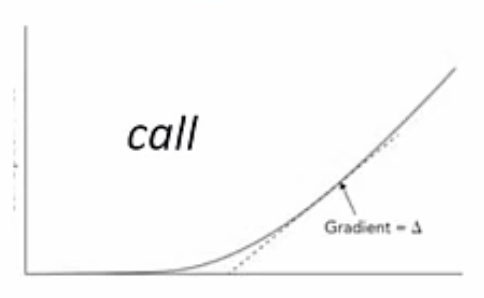
\includegraphics[width=0.7\textwidth]{value-call.jpg}
 			\caption{Стоимость (value) Call}
 			 	\label{model}
 	\end{subfigure}
 	 	\begin{subfigure}{.45\textwidth}
 		\centering
 		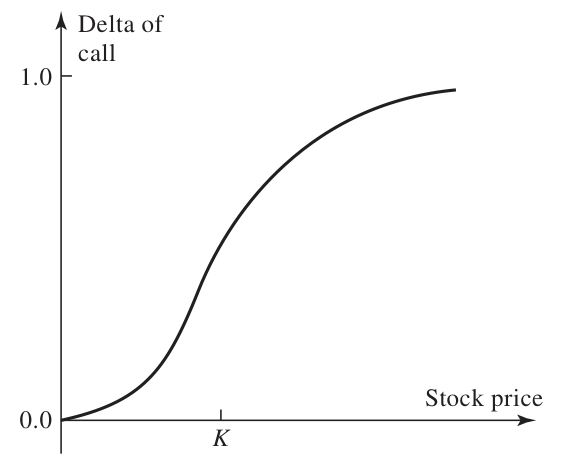
\includegraphics[width=0.7\textwidth]{delta-call.jpeg}
 		\caption{Зависимость Дельты от сток цены}
 			\label{model}
 		\end{subfigure}
 
 	\caption{Call опцион}
 	\label{model}
 \end{figure}
\bigskip

%\bigskip
  \begin{figure}[h]
	\centering
	\begin{subfigure}{.5\textwidth}
		\centering
		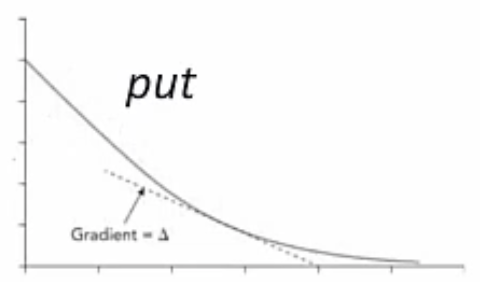
\includegraphics[width=0.7\textwidth]{value-put.jpg}
		\caption{Стоимость (value) Put}
		\label{model}
	\end{subfigure}
	\begin{subfigure}{.47\textwidth}
		\centering
		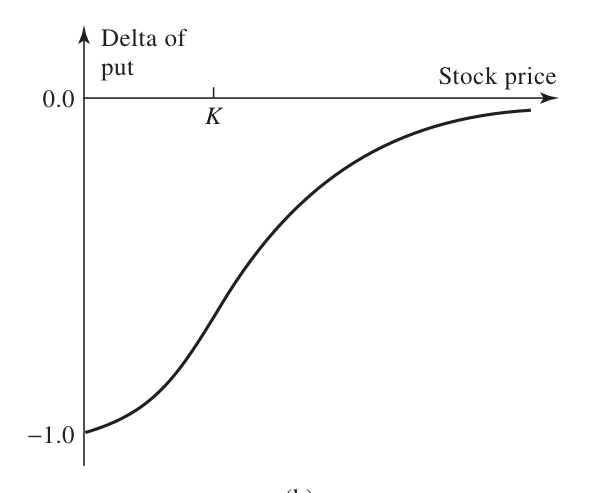
\includegraphics[width=0.7\textwidth]{delta-put.jpeg}
		\caption{Зависимость Дельты от сток цены}
		\label{model}
	\end{subfigure}
	
	\caption{Put опцион}
	\label{model}
\end{figure}
%\end{itemize}
 
% \setcounter{section}{1}
% \value{counter}

 
%\setcounter{section}{2} 
%\setcounter{subsection}{1} 
\subsection{Тета}

 \textbf{Тета ($\Theta$)} - мера чувствительности стоимости (value) дериватива к изменению времени до экспирации. Математическое выражение определения:
 $$\Theta = \dfrac{\partial f}{\partial t},$$ где $f$ - стоимость (value) дериватива, $t$ - время. 
 
\begin{itemize}
\item \underline{В чем особенность Теты?} Параметры других греков являются стохастическими параметрами, например, цена базового актива или волатильность и т.д., а у Теты время - детерминированный параметр.
 
 \item Тету для обычного ванильного Call или Put опциона легко вычислить с помощью формулы Блэка-Шоулза-Мёртона, взяв производную дериватива по времени. Формулы выглядят следующим образом:
 
 $$\Theta_{call} = -\dfrac{S_0 N'(d_1) \sigma}{2 \sqrt{T}} - rKe^{-rT}N(d_2),$$
 $$\Theta_{put} = -\dfrac{S_0 N'(d_1) \sigma}{2 \sqrt{T}} + rKe^{-rT}N(-d_2),$$
 $$N'(x) = \dfrac{1}{\sqrt{2\pi}} \exp{-\frac{x^2}{2}}$$
 
 \item Если мы разделим формулы выше на 365, то получим, на сколько изменяется стоимость (value) дериватива за один день.
 
\item При изменении времени стоиомсть (value) дериватива, как правило, уменьшается. Чем больше времени, тем больше возможностей для исполнения опциона, тем выше его стоимость (value). Чем меньше времени до экспирации, тем меньше возможностей для исполнения, значит, тем меньше возможностей оказаться в области in-the-money в момент экспирации, следовательно, тем меньше стоимость (value).

\item По графику Тета для Call опциона является величиной отрицательной. Для Put опциона в некоторых случаях Тета может быть положительной (для deep in-the-money).


  \begin{figure}[h]
	\centering
	\begin{subfigure}{.49\textwidth}
		\centering
		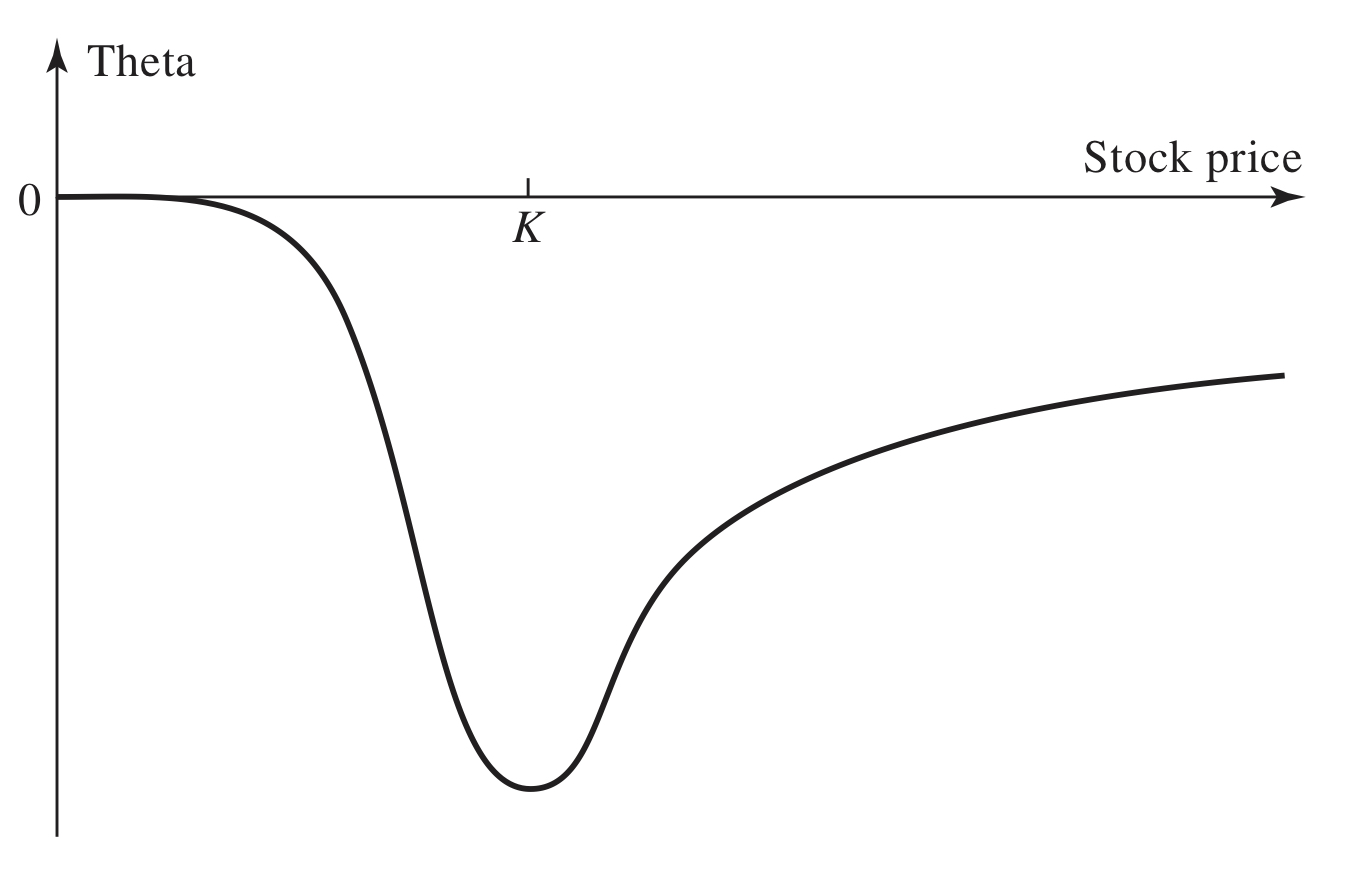
\includegraphics[width=0.7\textwidth]{thetta-stock.jpg}
		\caption{Зависимость Теты от сток цены}
		\label{model}
	\end{subfigure}
	\begin{subfigure}{.5\textwidth}
		\centering
		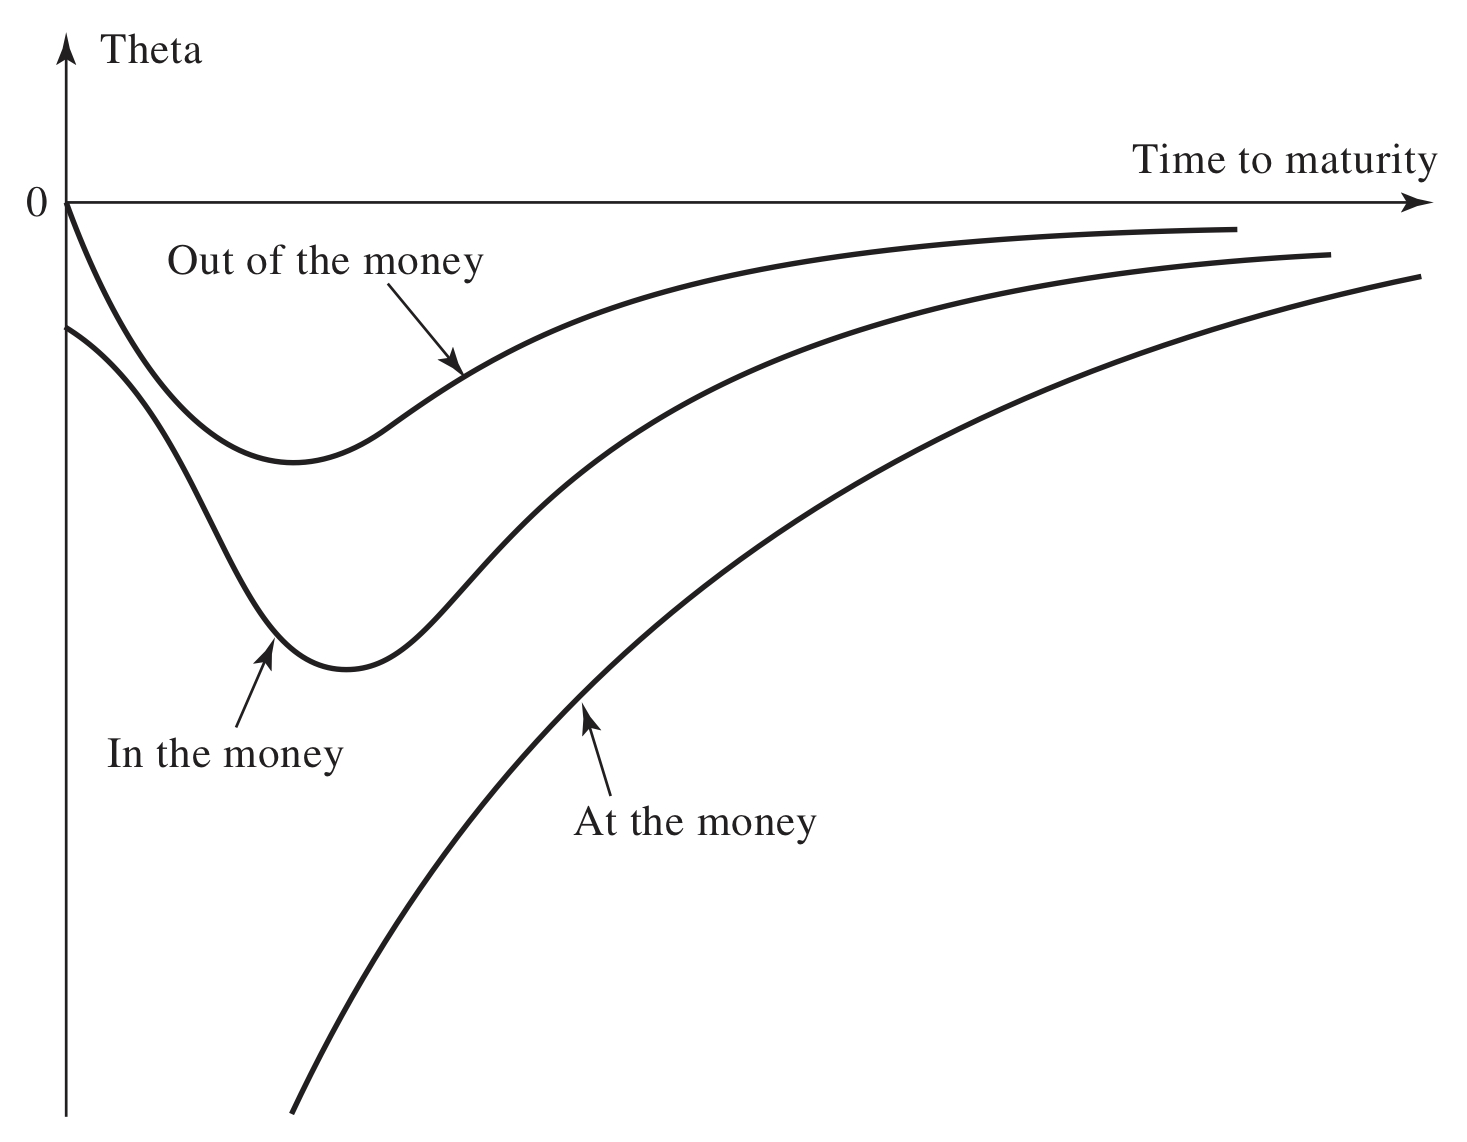
\includegraphics[width=0.7\textwidth]{thetta-time.jpg}
		\caption{Зависимость Теты от времени}
		\label{model}
	\end{subfigure}
	
	\caption{Графики Теты для Call опциона}
	\label{model}
\end{figure}
%\newpage
Сформулируем вкратце свойства Теты, исходя из графиков. \\
\underline{Свойства Теты:}

\item Тета принимает отрицательные значения.
\item Тета меняется при изменении цены базового актива и с течением времени.
\item Больше всего Тета для at-the-money опционов по сравнению с out-of-the-money и in-the-money опционами.
\item  При приближении к дате экспирации опциона value Теты увеличивается в абсолютном значении.
\item Для in-the-money Put опциона Тета может быть положительной.

\item На графике изменения Теты от цены мы видим, что если цена уходит в регион deep in-the-money для Put опциона, то Тета принимает положительные значения.


\begin{figure}[h]
	\centering
	\begin{subfigure}{.49\textwidth}
		\centering
		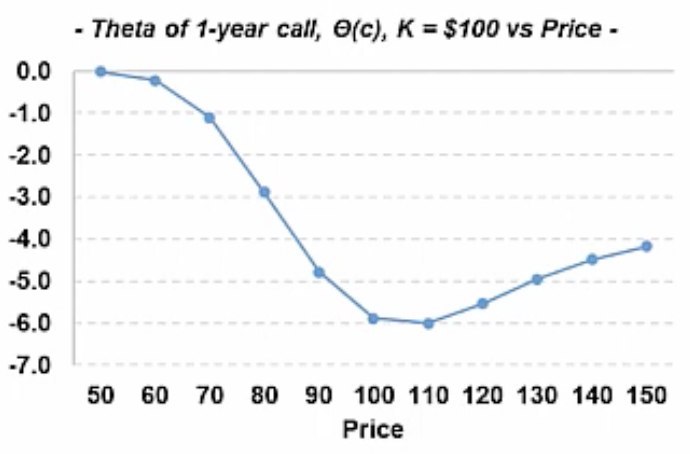
\includegraphics[width=0.7\textwidth]{theta-call-price.jpg}
		\caption{Зависимость Теты от цены для Call опциона}
		\label{model}
	\end{subfigure}
	\begin{subfigure}{.5\textwidth}
		\centering
		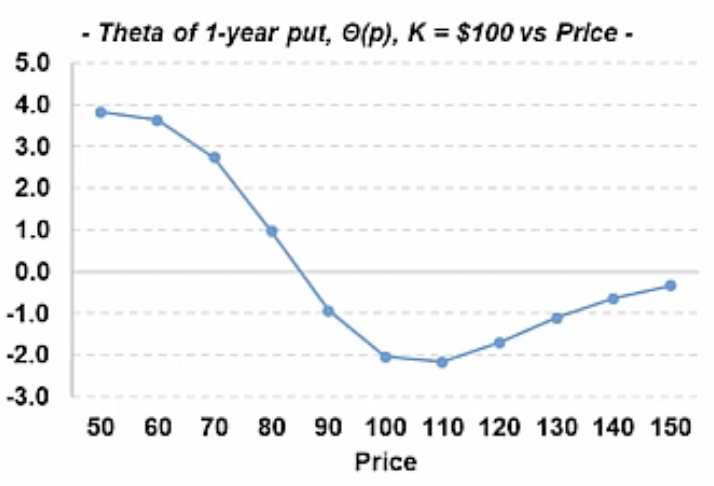
\includegraphics[width=0.7\textwidth]{theta-put-price.jpg}
		\caption{Зависимость Теты от цены для Put опциона}
		\label{model}
	\end{subfigure}
	
	\caption{Графики зависимости Теты от цены}
	\label{model}
\end{figure}

\end{itemize}

%\setcounter{section}{2} 
%\setcounter{subsection}{1} 
\subsection{Гамма}
 \textbf{Гамма ($\Gamma$) } - мера чувствительности Дельты к изменению цены базового актива. Математическое выражение определения: $$\Gamma = \dfrac{\partial \Delta}{\partial S},$$ где $S$ - цена базового актива. Альтернативная форма записи: $$\Gamma = \dfrac{\partial^2 f}{\partial S^2},$$ где $f$ - стоимость дериватива, $S$ - цена базового актива.

\begin{itemize}


\item \underline{Зачем нужен этот грек?} Дельта-нейтральные позиции таковыми являются и хеджируют портфель от изменения цены базового актива только в том случае, если эти изменения небольшие. В то же время Гамма помогает захеджировать портфель от относительно больших изменений в цене базового актива.

\item Формула для Гаммы для обычных ванильных Call и Put опционов выводится из формулы для Дельты и выглядит следующим образом:
$$\Gamma = \dfrac{N'(d_1)}{S_0 \sigma \sqrt{T}}$$
\item Из определения Гаммы следует, что для линейных пэйоффов Гамма нулевая (для самого базового актива, для форвардного инструмента Гамма равна нулю). \underline{Что следует отсюда?} Прежде всего, если ненулевая Гамма для всего портфеля, нам необходимо использовать инструменты с нелинейным пэйоффом, чтобы захеджировать Гамму нашего портфеля. Иными словами, мы не можем захеджировать портфель с ненулевой Гаммой по базовому  активу с помощью самого базового актива, форварда  на этот базовый актив и т.д., нам нужен, так сказать, опцион, чтобы это реализовать. \underline{Сколько нам понадобится опционов?} Количество опционов можно найти по следующей формуле. В портфеле должна быть добавлена позиция $\left(-\dfrac{\Gamma_p}{\Gamma_T}\right)$, где $\Gamma_p$ - Гамма существующего портфеля, $\Gamma_T$ - Гамма торгуемого опциона. Добавив такое количество опционов, мы получим нулевую Гамму по всему портфелю (по совокупной позиции). 




\end{itemize}



   \begin{figure}[h]
	\centering
	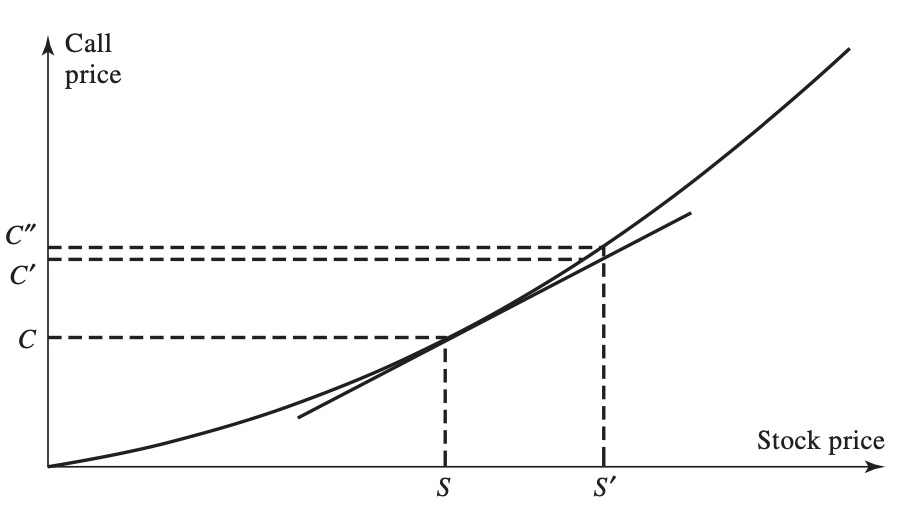
\includegraphics[width=0.5\textwidth]{option-price-profile.jpg}
	\caption{Профиль цены дериватива в зависимости от сток цены}
	\label{model}
\end{figure}


Чем больше выпуклость/вогнутость графика в точке, тем выше Гамма в данной точке для данного значения $S$, если мы нарисуем профиль цены дериватива в зависимости от сток цены.



\begin{figure}[h]
	\centering
	\begin{subfigure}{.49\textwidth}
		\centering
		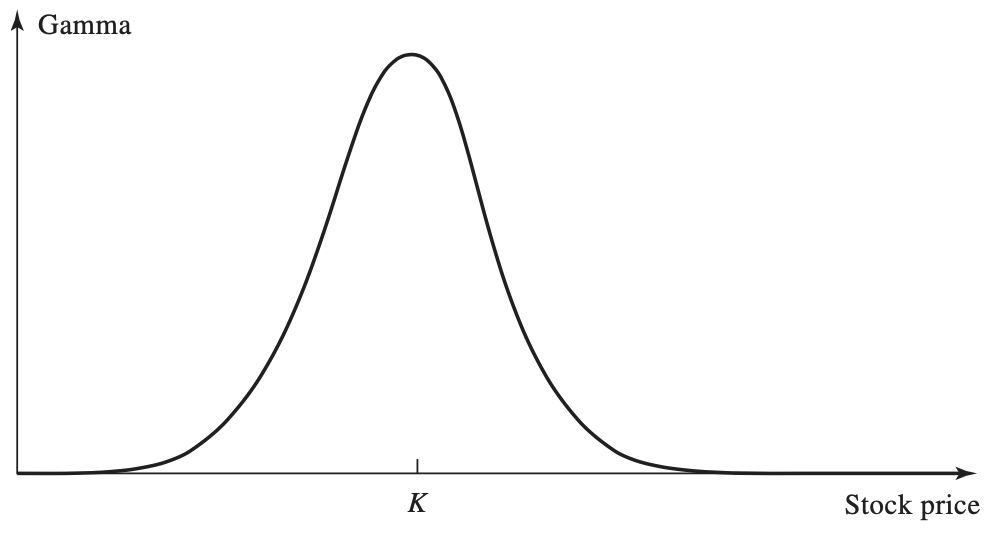
\includegraphics[width=0.7\textwidth]{gamma-stock.jpg}
		\caption{Зависимость Гаммы от сток цены}
		\label{model}
	\end{subfigure}
	\begin{subfigure}{.5\textwidth}
		\centering
		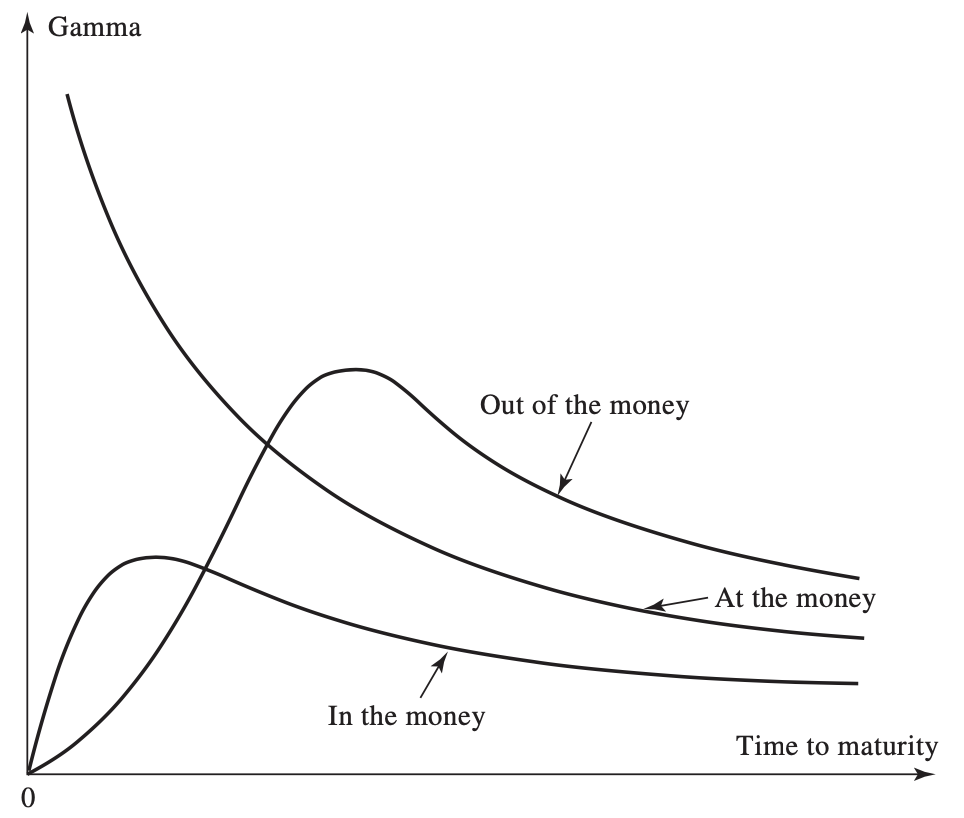
\includegraphics[width=0.7\textwidth]{gamma-time.jpg}
		\caption{Зависимость Гаммы от времени}
		\label{model}
	\end{subfigure}
	
	\caption{Графики зависимости Гаммы}
	\label{model}
\end{figure}


График колоколообразный, поскольку плотность нормального распределения имеет такую же форму.

%\end{itemize}

%\setcounter{section}{2} 
%\setcounter{subsection}{1} 
\subsection{Вега}
 \textbf{Вега ($\mathcal{V}$) } - мера чувствительности цены дериватива к изменению implied волатильности базового актива. Математическое выражение определения: $$\mathcal{V} = \dfrac{\partial f}{\partial \sigma},$$ где $f$ - стоимость (value) дериватива, $\sigma$ - implied волатильность базового актива.
 
 \textbf{Замечание:} Вега не название греческой буквы, обычно обозначается как большая $\nu$, так как внешне она напоминает букву $V$.
 
  \underline{Свойства Веги:}
 \begin{itemize}
 	
\item  Для европейского Call и Put опциона на бездивидендную акцию Вега рассчитывается по следующей формуле:
 $$\mathcal{V} = S_0 N'(d_1) \sqrt{T} $$
 


 	\item Профиль Веги напоминает профиль Гаммы с максимумом в цене страйк. 
 
%\item Из определения как опциона, так из формулы можно вывести, что максимум значения веги достигается в точке at-the-money, то есть непосредственно, когда спот цена равна страйк цене
 
 %Это понятно, так как для опциона, у которого спот цена находится в области страйка, чем больше волатильность, тем выше шанс оказаться как в области in-the-money, так и в области out-of-the-money, в этой точке влияние волатильности оказывается максимально.
 
% В то же время, е
\item Опционы наиболее чувствительны к изменениям в волатильности, когда мы находимся в области at-the-money. Если мы находимся в областях deep in-the-money или deep out-of-the-money, и даже если волатильность в этих точках увеличивается, то мы все равно при увеличенной волатильности остаемся в области in-the-money или out-of-the-money, то есть мы не переходим в другую область, и value опциона не меняется критическим образом. 

%В этих точках значение веги меньше, чем в точке at-the-money.
 
 \item При увеличении времени до экспирации Вега также увеличивается, при уменьшении - уменьшается.
 
 \begin{figure}[h]
 	\centering
 	\begin{subfigure}{.49\textwidth}
 		\centering
 		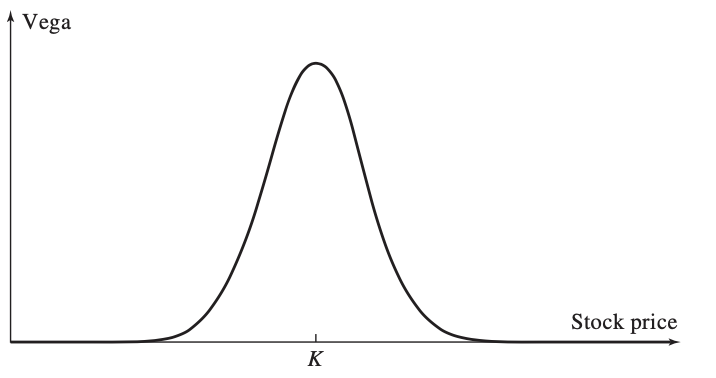
\includegraphics[width=0.7\textwidth]{vega-price.jpg}
 		\caption{Зависимость Веги от сток цены}
 		\label{model}
 	\end{subfigure}
 	\begin{subfigure}{.5\textwidth}
 		\centering
 		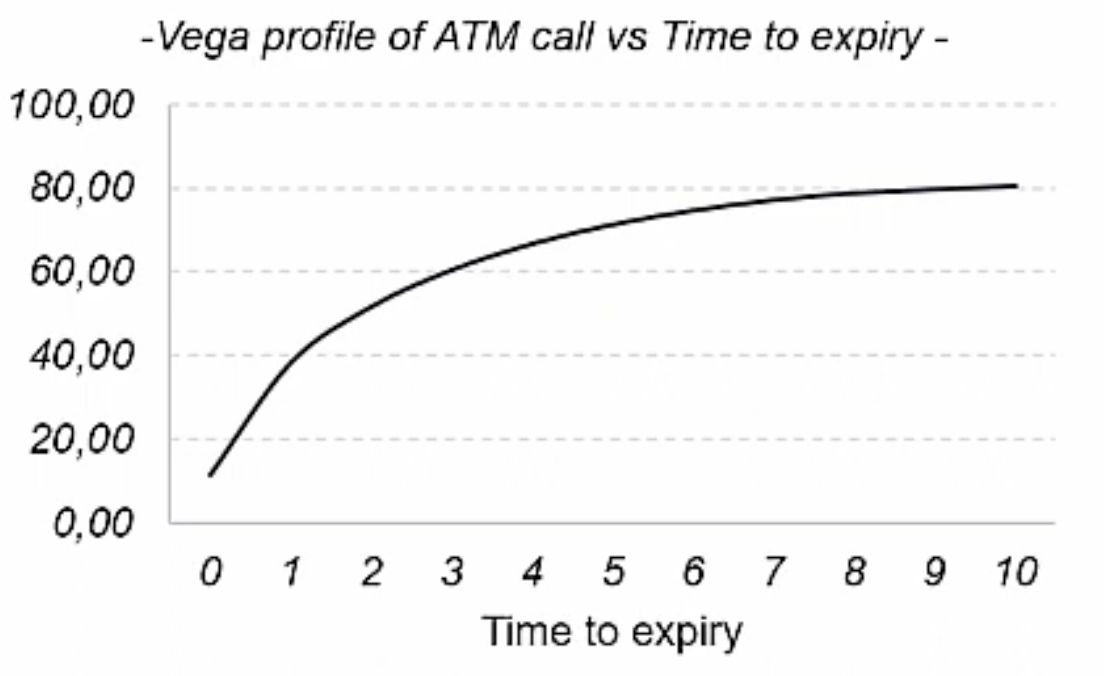
\includegraphics[width=0.7\textwidth]{vega-time.jpg}
 		\caption{Зависимость Веги от времени}
 		\label{model}
 	\end{subfigure}
 	
 	\caption{Графики зависимости Веги}
 	\label{model}
 \end{figure}
 
  \end{itemize}
 
 
 \subsection{Ро}
 \textbf{Ро ($\rho$) } - мера чувствительности стоимости (value) дериватива к изменению в значении безрисковой процентной ставки. Математическое выражение определения: $$\rho = \dfrac{\partial f}{\partial r},$$ где $f$ - стоимость (value) дериватива, $r$ - безрисковая процентная ставка.
 
 \begin{itemize}
 \item Для европейского Call и Put опциона на бездивидендную акцию Ро рассчитывается по следующим формулам:
 $$\rho_{call} = KTe^{-rT} N(d_2),$$
 $$\rho_{put} = -KTe^{-rT} N(-d_2)$$
 
 \item Для Call опциона профиль похож на профиль кумулятивной функции нормального распределения, для Put опциона - на смещенный профиль кумулятивной функции нормального распределения.
 
\item In-the-money Call и Put опционы более чувствительны к изменениям в процентных ставках, чем out-of-the-money опционы. Увеличение в значении процентных ставок вызывает большее увеличение цен (prices) in-the-money Call опционов по сравнению с ценами (prices) out-of-the-money Call опционов и большее снижение цен (prices) in-the-money Put опционов по сравнению с ценами (prices) out-of-the-money Put опционов.

   \end{itemize}
\newpage


   \begin{figure}[h]
	\centering
	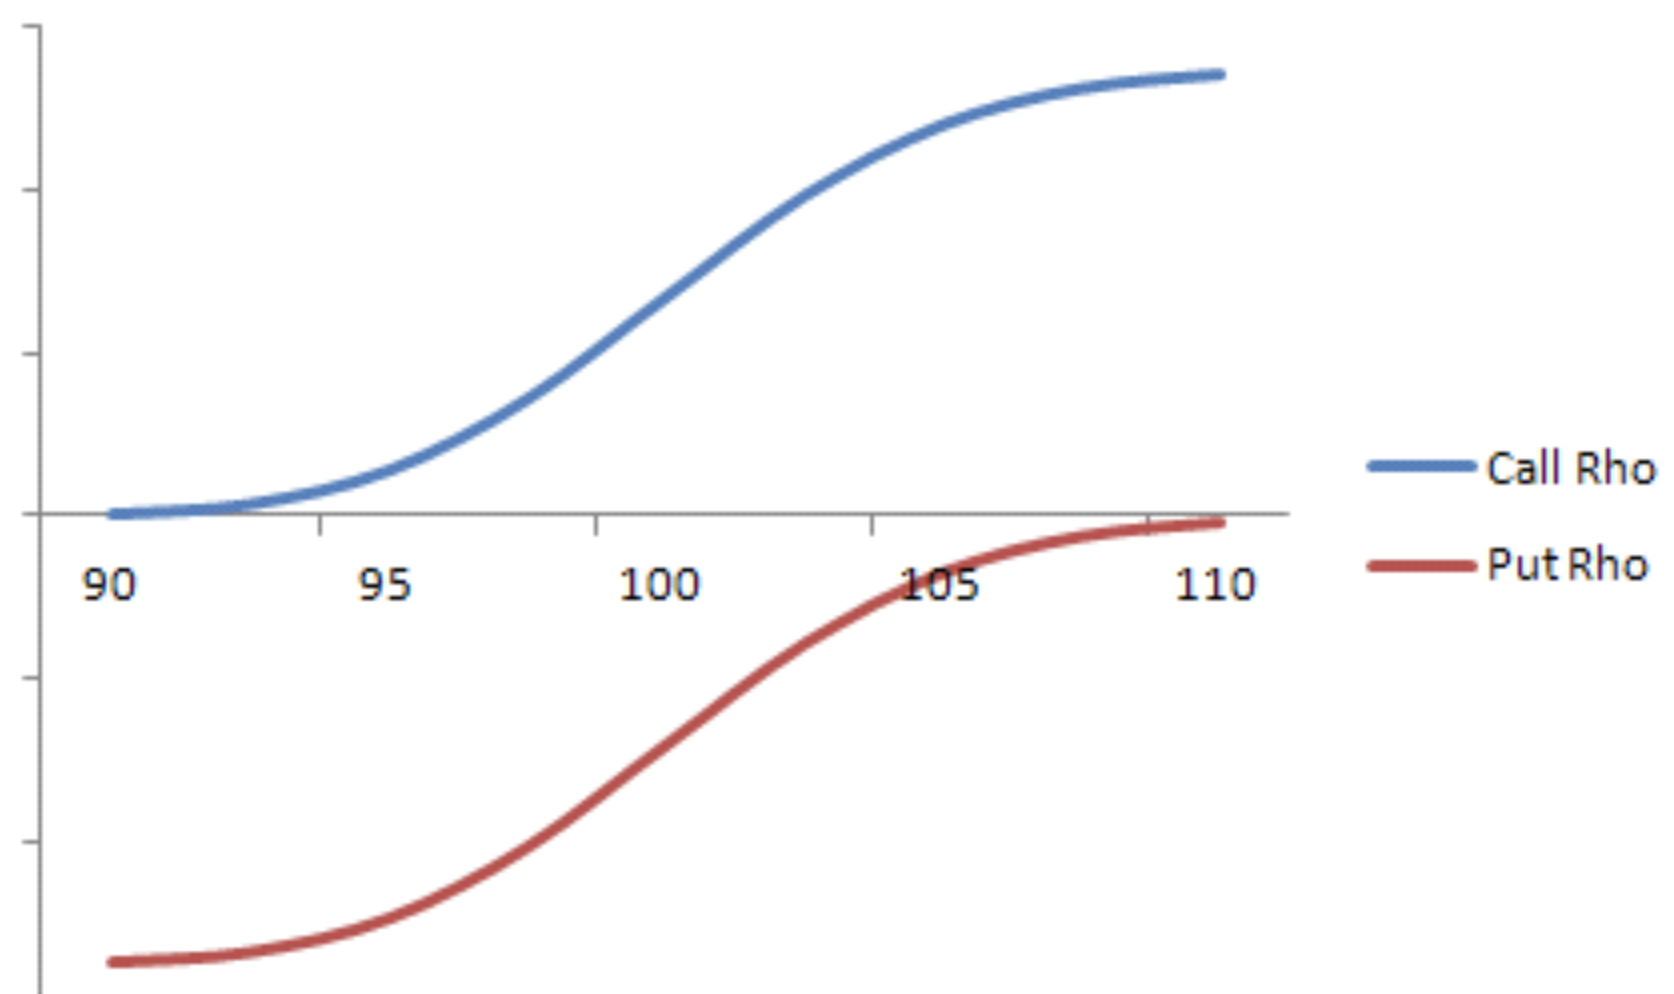
\includegraphics[width=0.5\textwidth]{rho-price1.jpg}
	\caption{Профиль Ро Call и Put опциона в зависимости от сток цены}
	\label{model}
\end{figure}

\section{Хеджирование на практике}
 \begin{itemize}
 	
\item \underline{Дельта-нейтральные позиции могут быть сравнительно легко созданы} (например, к портфелю опционов может быть добавлен базовый актив и линейный пэйофф).


\item \underline{Не всегда легко найти деривативы по разумным ценам для того, чтобы нейтрализовать Гамму и}

\underline{Вегу}. Нам необходим нелинейный пэйофф, но инструменты с нелинейным пэйоффом достаточно дорогие для целей хеджирования, отсюда возникает вопрос и достаточно высоких транзакционных издержек.

\item Из практики дельта-нейтральность портфеля мониторится на ежедневной основе, чуть реже происходит управление Гаммой и Вегой портфеля.

\item Гамма и Вега максимальны для at-the-money опционов и минимальны для
deep in-the-money и deep out-of-the-money. 

%Дело в том что когда опцион продается или покупается (обычно это происходит для атм опционов) но с течением времени цена уходит либо в облсть itm и otm с высокой вероятностью соотвественно гамма и вега для данных опционов снижаются автоматически и это хорошо в данном случае даже не требуются усилия с точки зрения хеджирования

\item Помимо мониторинга и управления греками, ещё одним инструментом управления прибыли и убытков портфеля является \underline{сценарный анализ}.


\item Ещё один технический аспект управления греками портфеля: \underline{установление лимитов для каждого} \underline{из греков}. Например, если лимит на Вегу утсановлен как 100 тысяч долларов за 1 процент, то это не означает, что мы должны добиваться нулевой Веги, но мы должны придерживаться следующего: при изменении волатильности на 1\% стоимость (value) нашего портфеля вследствие этого изменения должна меняться не больше, чем на 100 000 долларов.

\item \underline{Преимущество на стороне больших финансовых организаций}, поскольку они обладают существенной экономией от масштаба на данном рынке. Дело в том, что если у нас 10 инструментов в портфеле, то транзакционные издержки на хеджирование этого портфеля распределяются по этим 10 транзакциям, если же у нас 10 тысяч транзакций в портфеле, соответственно, издержки на хеджирование этого портфеля распределяются на 10 тысяч транзакций, что, очевидно, более приемлемо с точки зрения абсолютного выражения транзакционной издержки.

\item \underline{На больших объемах начинает вступать в силу закон больших чисел}: где-то отклонились в $+$, где-то в $-$ по тому или иному греку, но, в целом, у нас общая позиция не так сильно может меняться, особенно если корреляция между различными инструментами портфеля отрицательна или меньше единицы, в таком случае компонеты портфеля с точки зрения хеджирования благотворно влияют на общую позицию по портфелю.


  \end{itemize}

\section{Соотношение между греками}

Рассмотрим уравнение в частных производных Блэка-Шоулза-Мёртона. Если заменим производные в данном уравнении в частных производных на соответствующих греков, то получим:
$$r\Pi = \Theta + r S\Delta + 0.5\sigma^2S^2\Gamma,$$
где $r$ - безрисковая процентная ставка,
$\Pi$ - цена опциона или value портфеля, $\Theta$ -  Тетта опциона, $S$ - цена базового актива, $\Delta$ - Дельта опциона, $\sigma^2$ - дисперсия базового актива , $\Gamma$ - Гамма опциона.

Это соотношение дает возможность для дельта-нейтрального портфеля записать соотношение на изменение стоимости (value) портфеля в зависимости от изменения цены базового актива. Поскольку имеем квадратичное соотношение, то график данного изменения представляет собой параболу. Отсюда получим важное соотношение:
 
\begin{figure}[h]
	\centering
	\begin{subfigure}{.49\textwidth}
		\centering
		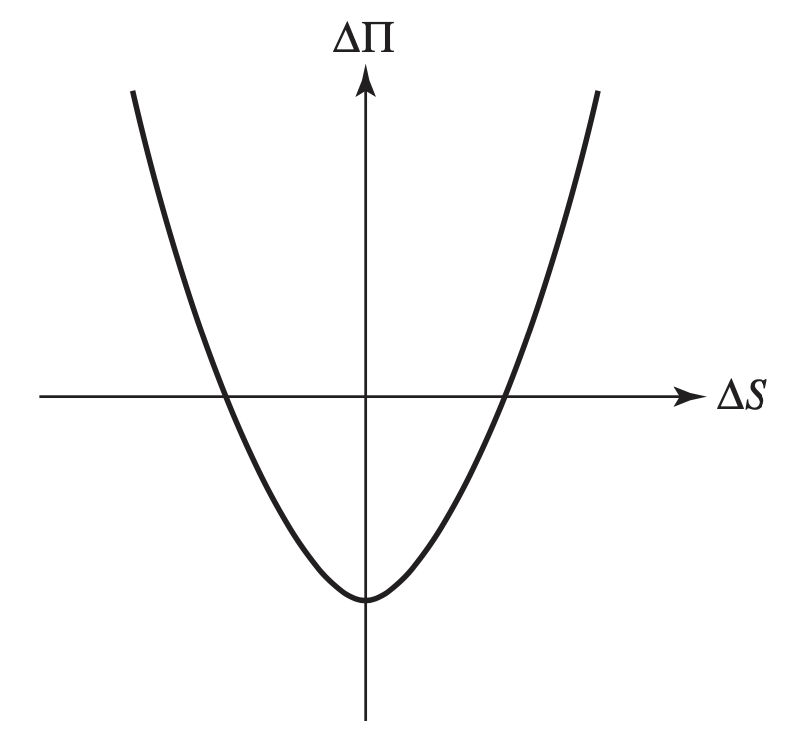
\includegraphics[width=0.7\textwidth]{pos-gamma.jpg}
		\caption{Зависимость $\Delta\Pi$ от $\Delta S$ при положительной $\Gamma$}
		\label{model}
	\end{subfigure}
	\begin{subfigure}{.5\textwidth}
		\centering
		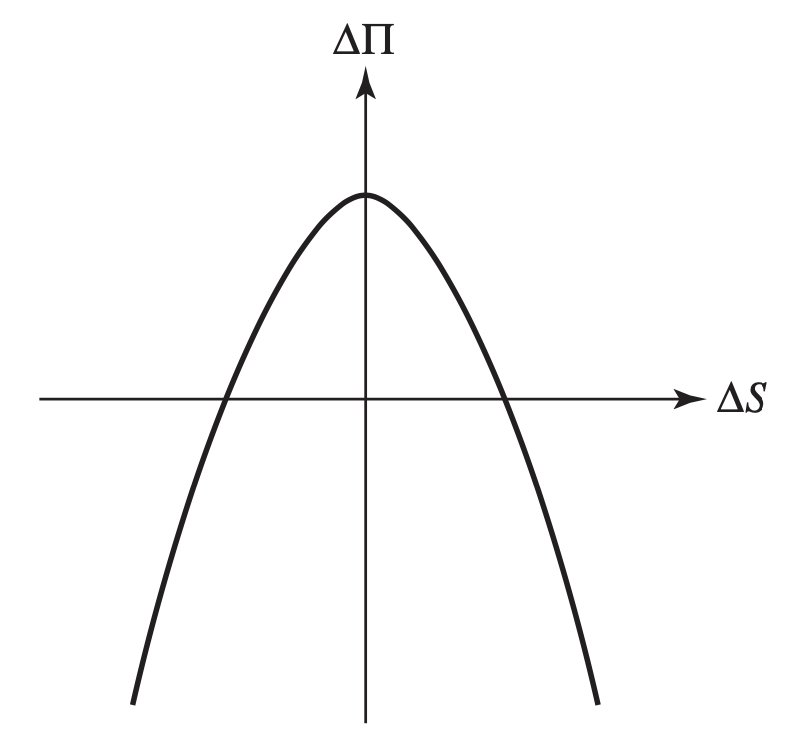
\includegraphics[width=0.7\textwidth]{neg-gamma.jpg}
		\caption{Зависимость $\Delta\Pi$ от $\Delta S$ при отрицательной $\Gamma$}
		\label{model}
	\end{subfigure}
	
	\caption{Графики зависимости для дельта-нейтрального портфеля}
	\label{model}
\end{figure}

\section{Портфель}
\subsection{Греки для всего портфеля}

Выше мы рассматривали греков, расчитываемых от отдельных опционов.

\underline{Как рассчитать грек для всего портфеля из опционов, базовых активов и других деривативов?}

Вспомним свойство производной функции: производная линейной комбинации функций является линейной комбинацией производных этих функций. Греки представляют собой нечто иное, как производные по рыночным параметрам, поэтому мы можем использовать это свойство и для греков.

Рассмотри в качестве примера Дельту портфеля:
 $$\Delta_{port} = \sum_{i=1}^{n}w_i\Delta_i,$$
 где $\Delta_i$ - Дельта каждой компоненты, $w_i$ - веса данных компонент в общем портфеле.
 Дельта портфеля представляет собой ожидаемое изменение общей позиции по портфелю в случае небольшого изменения цены базового актива.
Аналогично, можно проделать то же самое и для других греков.

\subsection{Страхование портфеля с помощью создания синтетической позиции в Put опционе}

Предположим, что у нас есть портфель под управлением asset менеджера. Главный интерес asset менеджера - застраховаться от падения стоимости (value) данного портфеля в случае неблагоприятных рыночных условий.

\underline{Какой дериватив предоставляет страховку от падения цены базового актива?} Это Put опцион. 
\begin{itemize}
\item \underline{Идея:} либо купить Put опционы на рынке на данный портфель, либо синтетически создать Put опцион на данный портфель. На рынке не всегда могут быть нужные нам опционы (например, опционы на индекс, за которым следует портфель), так как портфель может быть уникален по своим характеристикам. Поэтому зачастую до 80-х годов прошлого века управляющие портфелями использовали такой подход, как создание позиции в Put опционе на портфель синтетически.
 
 %идея в том чтобы путем продажи и покупки частей портфеля мимикрировать, то есть реплицировать пут синетически с помощью реплицирования дельты пута
 
 \item Если asset менеджер добивается того, что Дельта, получившаяся путем продажи/покупки частей портфеля, совпадает с Дельтой Put опциона, то он тем самым автоматически создает синтетическую позицию в Put опционе.
 
 \item \underline{Издержки по данной стратегии} дают стоимость (value) Put опциона за применение подобной стратегии. Покупка происходит на рынке, идущем вверх, а продажа портфеля - на снижающемся рынке.
 
 \item \underline{Что же произошло?} После черного понедельника, когда использование подобных синтетических Put опционов сделало достаточно глубокое неуправляемое падение, оно тем самым доказало слабость подобных стратегий страхования портфеля. \underline{Почему произошло падение?} Дело в том, что рынок упал, затем рынок дальше стал падать путем срабатывания алгоритмов "продавай на снижающемся рынке"\ , и все больше участников рынка стали продавать свои активы, что еще больше усугубило падение. В конечном счете, падение достигло катастрофических масштабов.
 
\end{itemize}


\end{document}
